\documentclass{beamer}
%
% Choose how your presentation looks.
%
% For more themes, color themes and font themes, see:
% http://deic.uab.es/~iblanes/beamer_gallery/index_by_theme.html
%
\mode<presentation>
{
  \usetheme{default}      % or try Darmstadt, Madrid, Warsaw, ...
  \usecolortheme{default} % or try albatross, beaver, crane, ...
  \usefonttheme{default}  % or try serif, structurebold, ...
  \setbeamertemplate{navigation symbols}{}
  \setbeamertemplate{caption}[numbered]

} 

\setbeamertemplate{footline}[text line]{%
  \parbox{\linewidth}{\vspace*{0pt}
    \begin{flushright}Copyright \textcopyright\ 2016 \insertshortauthor.\end{flushright}}}

\usepackage[english]{babel}
\usepackage[utf8x]{inputenc}
\usepackage{color}

\usepackage{tikz}
\usetikzlibrary{mindmap,trees}


\linespread{1.3}
\definecolor{links}{HTML}{2A1B81}
\hypersetup{colorlinks,linkcolor=,urlcolor=links}

\title[]{Operations research with Julia and JuMP}
\author{Pedro Belin Castellucci}
\date{February, 2016}


\begin{document}

\setbeamercolor{title}{fg=black}
\setbeamercolor{frametitle}{fg=black}


\begin{frame}
  \titlepage
\end{frame}


\section{Introduction}

\begin{frame}{Mathematical programming}

  \begin{figure}[htpb]
    \centering
  \scalebox{0.7}{
    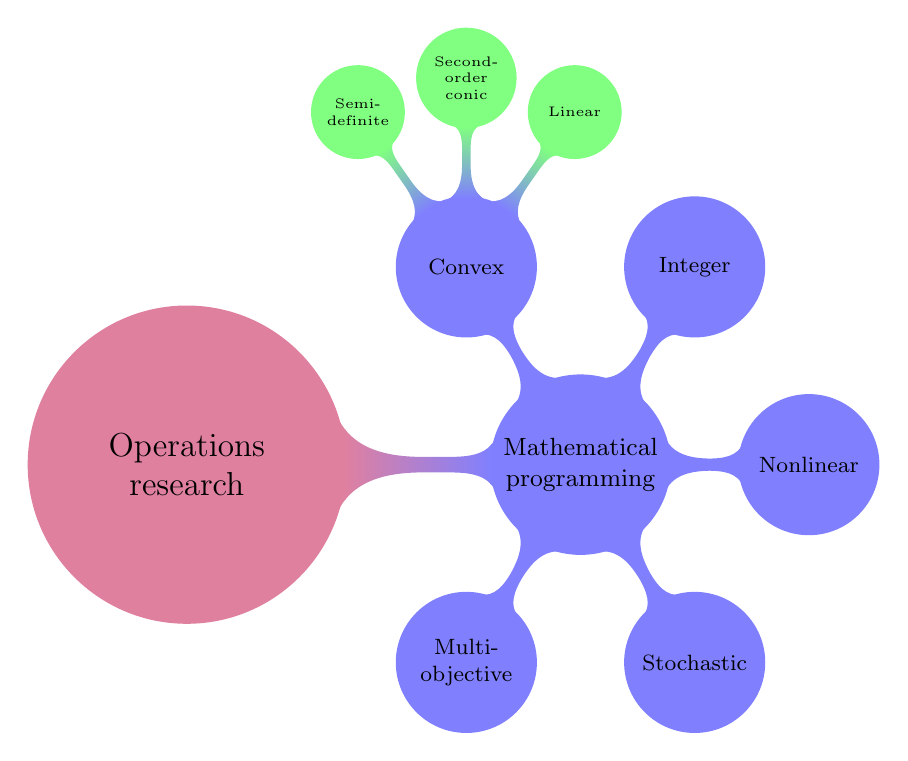
\begin{tikzpicture}

%      \pgflowlevel{\pgftransformscale{0.7}}
      
      \path[mindmap, concept color=purple!50, text=black]
      node[concept] {Operations \\research}
      [clockwise from=0]
      child[concept color=blue!50] {
        node[concept] {Mathematical programming}
        [clockwise from=120]
        child { node[concept] {Convex}
          child [concept color=green!50, grow=125]{ node[concept] {Semi-definite} } 
          child [concept color=green!50, grow=90] {node[concept] {Second-order conic}}
          child [concept color=green!50, grow=55] {node[concept] {Linear}}
        }
        child { node[concept] {Integer} }
        child { node[concept] {Nonlinear} }
        child { node[concept] {Stochastic} }
        child { node[concept] {Multi-objective} }
      };
    \end{tikzpicture}
  }
  \caption{Information from \href{https://en.wikipedia.org/wiki/Mathematical_optimization}{this link}.}
  \end{figure}

\end{frame}


\begin{frame}{Which can JuMP handle?}

  \begin{figure}[htpb]
    \centering
  \scalebox{0.7}{
    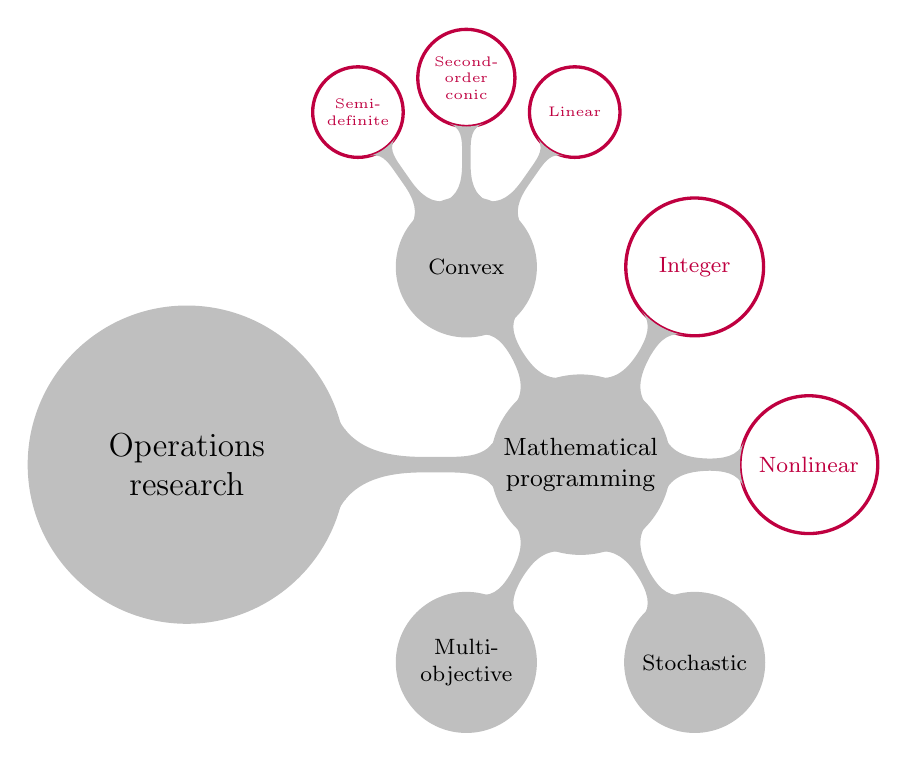
\begin{tikzpicture}

%      \pgflowlevel{\pgftransformscale{0.7}}
      
      \path[mindmap, concept color=gray!50, text=black]
      node[concept] {Operations \\research}
      [clockwise from=0]
      child[concept color=gray!50] {
        node[concept] {Mathematical programming}
        [clockwise from=120]
        child { node[concept] {Convex}
          child [concept color=gray!50, grow=125]{ node[draw, circle, purple] {Semi-definite} } 
          child [concept color=gray!50, grow=90] { node[draw, circle, purple] {Second-order conic}}
          child [concept color=gray!50, grow=55] { node[draw, circle, purple] {Linear}}
        }
        child { node[draw, circle, purple] {Integer} }
        child { node[draw, circle, purple] {Nonlinear} }
        child { node[concept] {Stochastic} }
        child { node[concept] {Multi-objective} }
      };
    \end{tikzpicture}
  }
  \caption{For JuMP documentation click on \href{http://www.juliaopt.org/JuMP.jl/0.15/}{this link}.}
  \end{figure}

\end{frame}


\begin{frame}
  \begin{center}
    Introduction to Julia programming
    \end{center}
\end{frame}


\begin{frame}
  \begin{quote}\footnotesize

  ``We want a language that’s \textcolor<2->{red}{open source}, with a \textcolor<3->{red}{liberal license}. We want \textcolor<4->{red}{the speed of C} with the \textcolor<5->{red}{dynamism of Ruby}. We want a language that’s \textcolor<6->{red}{homoiconic}, with \textcolor<7->{red}{true macros like Lisp}, but with obvious, \textcolor<8->{red}{familiar mathematical notation like Matlab}. We want something \textcolor<9->{red}{as usable for general programming as Python}, \textcolor<10->{red}{as easy for statistics as R}, \textcolor<11->{red}{as natural for string processing as Perl}, \textcolor<12->{red}{as powerful for linear algebra as Matlab}, \textcolor<13->{red}{as good at gluing programs together as the shell}. Something that is \textcolor<14->{red}{dirt simple to learn}, yet keeps the most serious hackers happy. We want it \textcolor<15->{red}{interactive} and we want it \textcolor<16->{red}{compiled}.
\newline
\visible<17->{(Did we mention it should be as fast as C?)}''\\
  \href{http://julialang.org/blog/2012/02/why-we-created-julia}{Jeff Bezanson, Stefan Karpinski, Viral Shah, Alan Edelman (2012)}
     \end{quote}
\end{frame}


\begin{frame}
  \frametitle{How fast is it? According to \href{http://julialang.org/benchmarks/}{this link}.}
  \begin{figure}[htpb]
    \centering
    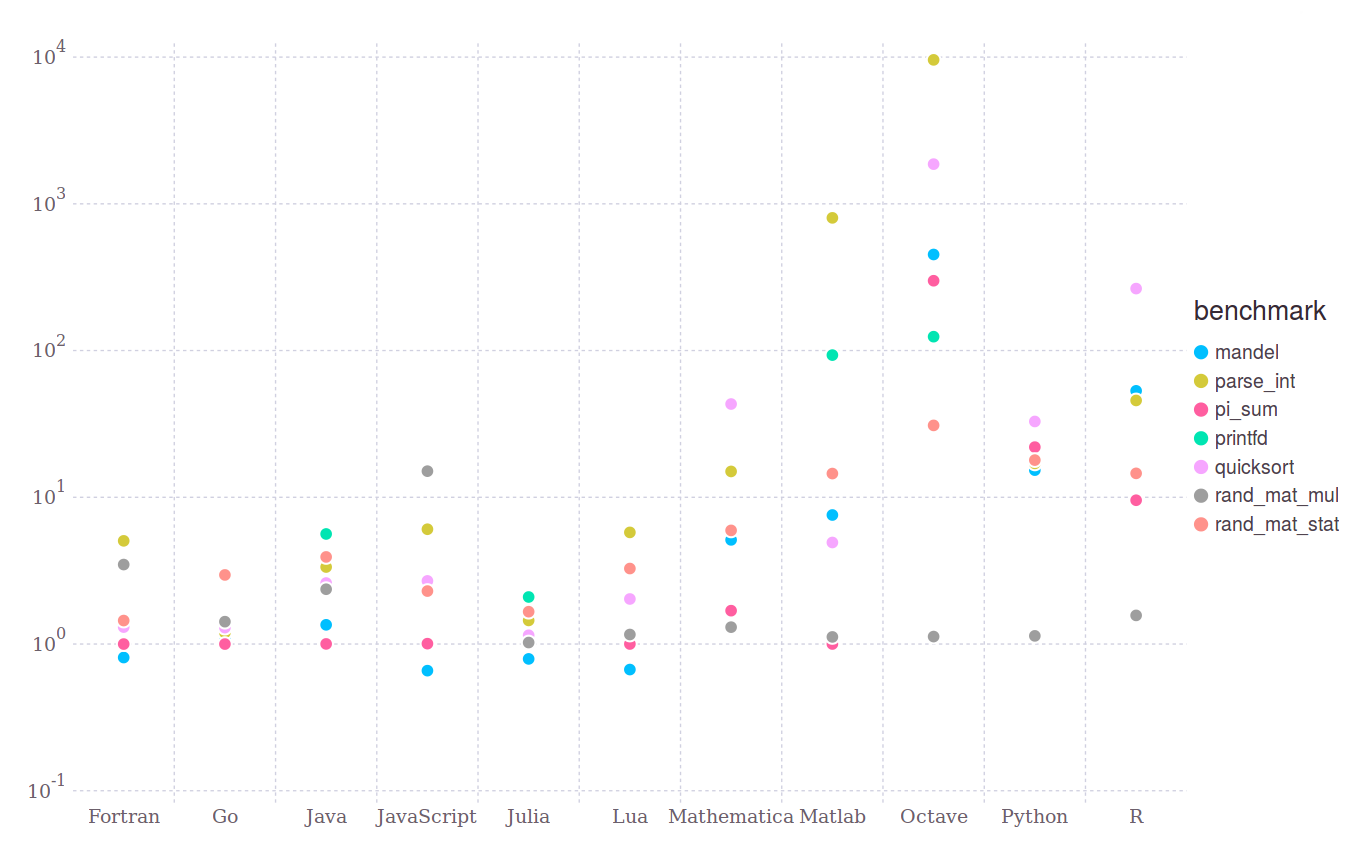
\includegraphics[scale=0.2]{BenchmarkImage.png}
    \caption{Speed relative to C smaller is better (C performance is 1.0).}
    \label{fig:benchmark}
  \end{figure}
\end{frame}

\begin{frame}{Who is using Julia?}
  \begin{itemize}\footnotesize
  \item[] Stanford University. Introduction to Multidisciplinary Design Optimization (Prof. Mykel J. Kochenderfer).
  \item[] MIT. Integer Programming and Combinatorial Optimization (Prof. Juan Pablo Vielma).
  \item[] MIT. Optimization Methods (Prof. Dimitris Bertsimas and Dr. Phebe Vayanos).
  \item[] University at Buffalo. Linear Programming (Prof. Changhyun Kwon).
  \item[] “Sapienza” University of Rome. Operations Research (Giampaolo Liuzzi).
    \item[] University of South Florida. Nonlinear Optimization and Game Theory (Prof. Changhyun Kwon).
  \end{itemize}
\end{frame}


\begin{frame}{What can I do with Julia?}
  \begin{itemize}\footnotesize
  \item[] Simple Audio IO in Julia (AudioIO).
  \item[] A neural network (BackpropNeuralNet).
  \item[] Support vector machines (LIBSVM, LIBLINEAR).
  \item[] Machine learning (MachineLearning).
  \item[] Bioinformatics and Computational Biology (Bio).
  \item[] Curve fitting (CurveFit).
  \item[] Describe and model financial markets (FinancialMarkets).
  \item[] Black-box optimization (BlackBoxOptim).
  \item[] Combinatorics (Combinatorics).
  \item[] Evolutionary and genetic algorithms (Evolutionary).
  \item[] Gurobi, GLPK, CPLEX, Cbc, Clp CoinOptServices, JuMP.
  \item[] \href{http://pkg.julialang.org/}{And more...}
  \end{itemize}
\end{frame}

\begin{frame}{What we will do?}
  \begin{itemize}
  \item[] Basic Julia programming.
  \item[] Explore JuMP for mixed integer linear problems.
  \end{itemize}
\end{frame}

\begin{frame}
  \href{https://www.cs.utexas.edu/users/EWD/transcriptions/EWD08xx/EWD831.html}{Why numbering should start at zero}?
  \pause
  ``I don't know how many of you have ever met Dijkstra, but you probably know that arrogance in computer science is measured in nano-Dijkstras.'' (Alan Kay)
\end{frame}

\begin{frame}
  \frametitle{Installing Julia}

  \begin{block}{On Linux/Ubuntu:}
  sudo add-apt-repository ppa:staticfloat/juliareleases

  sudo apt-get update

  sudo apt-get install julia  
  \end{block}
  \vspace{2cm}
  For other platforms check \href{http://julialang.org/downloads/platform.html}{this link}.
\end{frame}

% \begin{frame}
%   Implement a function with parameter $n$ to print the first $n$ prime numbers. 
% \end{frame}

% \begin{frame}
%   Implement an algorithm to count the number of words in a file.
% \end{frame}

\end{document}


%%% Local Variables:
%%% mode: latex
%%% TeX-master: t
%%% End:
